\chapter{Opis projektnog zadatka}
		
		
		Cilj ovog projektnog zadatka je razviti programsku podršku za stvaranje web aplikacije „Poliklinika za rehabilitaciju“. Rehabilitacija od bolesti, ozljeda i operacija je složen i osjetljiv proces koji zahtjeva disciplinu i detaljan plan kojeg se pacijent mora držati. Svaki pacijent je drugačiji i zahtjeva specifičnu njegu koju mu bolnica mora osmisliti i omogućiti. Danas se nalazimo u modernom dobu gdje tehnologija uvelike olakšava mnoge aspekte ljudskog života pa tako i oporavak pacijenata te motrenje njihovog napretka i prevencija potencijalnih novih ozljeda.\\
		
		U procesu oporavka određenim pacijentima je potreban doktor koji će propisati prikladnu dijetu, a nekim pacijentima je potreban samo trener koji će propisivati vježbe za svaki dan i motriti napredak te ponovno prilagođavati intenzitet vježbe s obzirom na trenutno stanje pacijenta. Na kraju postoje pacijenti kojima treba i doktor i trener koji će mu pomoći.\\
		
		Svakodnevni odlazak u bolnicu mnogim pacijentima nije najbolji put do oporavka. Većina pacijenata nije u dovoljno dobrom fizičkom stanju za putovanje u bolnicu i čekanje u redu. Također za bolnicu nije efikasno da primaju toliko pacijenata ako postoji lakši način kojim bi mogli komunicirati sa svojim pacijentima i dati im najbolje savjete bez stresa i požurivanja.\\
		
		Zbog ovih razloga stvorili smo aplikaciju koja bi omogućila stalnu komunikaciju između pacijenata, doktora i trenera. Doktor i trener ne mogu stalno biti s pacijentom i motriti ga, ali pomoći ove aplikacije pacijenti bi uvijek znali što moraju raditi, koliko i što smiju jest i imali bi osjećaj da je netko uvijek uz njih, a psihološka podrška je također vrlo bitna za pacijente.\\
		
		U aplikaciji, doktor bi imao mogućnost propisivanja dijete pacijentu, a trener bi mu zadavao točno definirane treninge za svaki dan.\\
		\newpage
		\noindent \textbf{REGISTRACIJA}
		
		Kako bi se mogla koristiti ova aplikacija budući korisnik se mora prvo registrirati tako da pošalje zahtjev za registraciju prilikom koje bira ulogu koju želi imati, a one su slijedeće:
		\begin{packed_item}
		\item \textbf{Klijent}
		\item \textbf{Doktor}
		\item \textbf{Trener}
		\end{packed_item}
		Prilikom svake registracije potrebno je unijeti:
		\begin{packed_item}
		\item \textbf{KorisničkoIme}
		\item \textbf{Ime}
		\item \textbf{Prezime}	
		\item \textbf{Loziku}
		\end{packed_item}
		Ukoliko se korisnik želi registrirati kao doktor ili trener potrebno je također dodatno priložiti:
		
		\begin{packed_item}
		\item \textbf{Sliku}
		\item \textbf{Mail}
		\item \textbf{Maskimalan broj korisnika(koje želi nadgledati)}	
		\end{packed_item}
	
		Da bi neregistrirani korisnik dobio prava doktora i trenera, administrator ga mora potvrditi.
		Svi registrirani korisnici imaju mogućnost mijenjanja podataka na svom profilu.\\
		
		\noindent \textbf{PROIZVODI}
		
		Svaka dijeta sastoji se od određenih proizvoda koje klijenti mogu konzumirati. Bitno je da i doktor i pacijent znaju što se točno nalazi u kojem proizvodu kako bi doktor što bolje osmislio dijetu i kako bi ju klijent  što bolje mogao pratiti.
		Popis proizvoda sa svim njihovim karakteristikama nalazit će se u bazi podataka. Svaki proizvod sadrži informacije o nutritivnim vrijednostima koje su definirane na 100 g, a to su:
		
			\begin{packed_item}
			\item \textbf{Energija}
			\item \textbf{Masnoće}
			\item \textbf{Zasićene masne kiseline}	
			\item \textbf{Ugljikohidrati}
			\item \textbf{Šećeri}
			\item \textbf{Bjelančevine}
			\item \textbf{Sol}
		\end{packed_item}
	
		Dodatno, svaki proizvod sadrži sliku, masu i prisutne alergene. Također, oni će biti raspoređeni u kategorije koje sadrže više različitih proizvoda sličnih karakteristika, kao što su na primjer tjestenina, proizvodi od mlijeka, meso, voće, povrće...\\
		
		\noindent \textbf{TRENINZI}\\
		Trening se sastoji od niza vježbi koje imaju određeno trajanje. Vježba je definirana sa:
		\begin{packed_item}
		\item \textbf{Slikom}
		\item \textbf{Opisom}
		\item \textbf{Informacijama o broju potrošenih kalorija u sat vremena u ovisnosti o 3 razine intenziteta vježbanja (lagano, normalno, teško)}
		\end{packed_item}
			
		\underbar{Klijent}
		ima mogućnost traženja i pronalazaka dostupnih(onih koji još nemaju popunjen maksimalan broj klijenata) doktora i trenera. Klijent može ostaviti recenziju s ocjenom i komentarom svom doktoru i treneru na koju oni mogu odgovoriti. Klijent, doktor i trener imaju mogućnost prekida suradnje. Sve kombinacije su moguće; da pacijent prekine suradnju s doktorom i trenerom ili samo jednim od njih. Kad pacijent prekine suradnju ima mogućnost biranja novog doktora i trenera, ali dok ih ne izabere on je u mogućnosti i dalje pratiti dijetu i trening koji su mu prije bili dodjeljeni.\\
		Klijent ima mogućnost unošenja slike bar koda proizvoda koje planira konzumirati, a aplikacija mu javlja(uzimajući u obzir i ostale konzumirane namirnice u tom danu) uklapa li se taj proizvod u dijetu za taj dan. Uz unošenje bar koda, klijent može i ručno odabrati proizvod i postaviti mu masu.\\
		
		\underbar{Doktor}
		svojim klijentima definira dijetu unoseći sve potrebne parametre. Dijeta se može definirati s ograničenjima na:\\
		\begin{packed_item}
		\item \textbf{određene proizvode}	
		\item \textbf{kategorije proizvoda}	
		\item \textbf{proizvode s nedopuštenim količinama sastojaka}	
		\item \textbf{dnevnim limitom za određene nutritivne vrijednosti proizvoda}
	\end{packed_item}
		
		Doktor ima mogućnost dodavanja novih proizvoda i kategorija proizvoda u bazu podataka.\\	
		
		\underbar{Trener}
		svojim klijentima definira vježbe koje trebaju odraditi. Definira točno koliko puta se koja vježba treba napraviti i kojim redosljedom ih mora raditi. Klijent će moći vidjeti sliku te vježbe i detaljan opis načina izvođenja vježbe. Trener određuje intenzitet vježbanja sukladno mogućnostima klijenta. S vremenom trener će mijenjati intenzitet kako bi oporavak prošao sa što manje ozljeda i najboljim rezultatima. Trener također ima pristup bazi podataka u koju može dodati nove vježbe.\\
		
		Administrator ima najveće ovlasti. On ima pristup bazi s  popisom kategorija proizvoda i vježbi i ima mogućnost uređivanja i brisanja. Također jedino on može potvrditi račun za doktora i trenera.\\
		
		\noindent \textbf{Nadogradnja}\\
		Aplikacija „Poliklinika za rehabilitaciju“ ostavlja mnogo prostora i mogućnosti za nadogradnju i proširenje. Korisno proširenje bilo bi omogućavanje slanja poruka između klijenata i doktora/trenera. Tako bi klijent mogao razriješiti postojeće nedoumice što prije, a ne bi ometao doktora/trenera slanjem poruka na privatni mobitel. Još jedno dobro proširenje bilo bi omogućavanje dogovora za pregled kod doktora, odnosno doktor bi mogao napomenuti klijentu da je vrijeme za pregled u bolnici i onda bi klijent u rasporedu izabrao slobodan termin koji mu najviše paše. Na taj način izbjegla bi se gužva i olakšao cijeli proces naručivanja kod doktora.\\
		
		Ova aplikacija je namijenjena širokom spektru ljudi. Napravljena je tako da bude laka za korištenje, intuitivna i jednostavna. Nema nepotrebnih funkcionalnosti koje bi dodatno zbunile korisnike, tako da ju svi mogu koristiti, od mladih do starih.
		
		\newpage
		
		\noindent \textbf{Slične aplikacije koje već postoje:}\\
		
		\underbar{REHAPTIX}
		\begin{figure}[h]
			\centering
			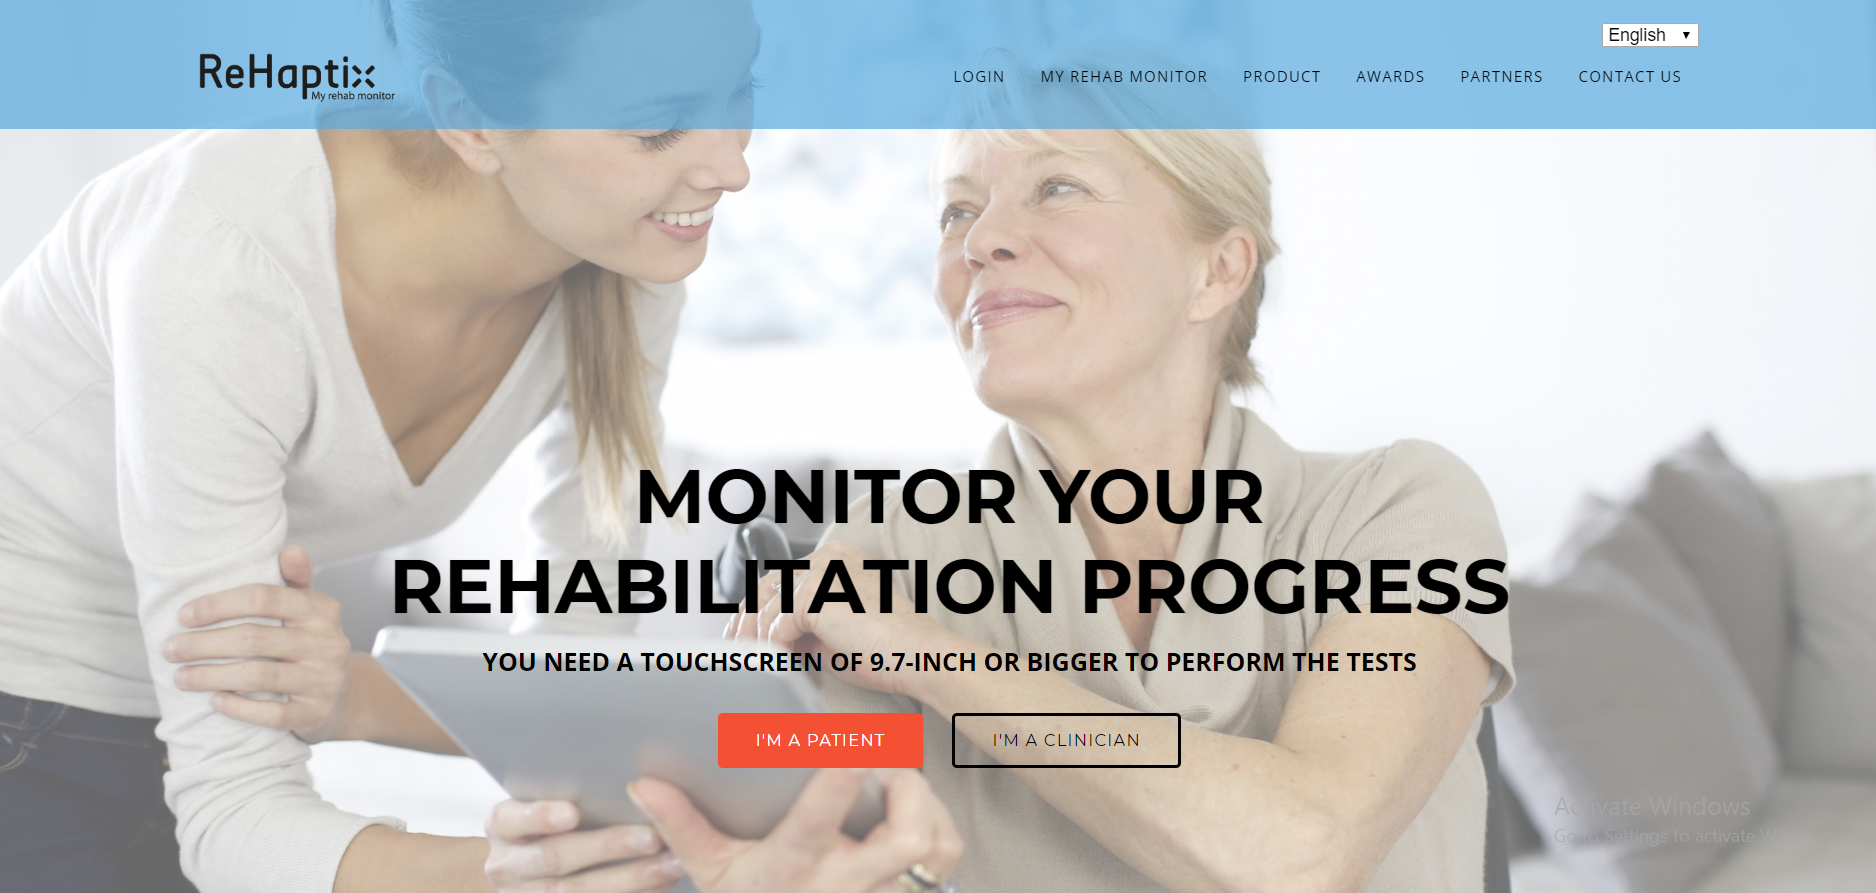
\includegraphics[scale=0.3]{slike/rehaptix1.png}
			\caption{Početna stranica}
		\end{figure}
	
	Ova aplikacija funkcionira jako slično kao i „Poliklinika za rehabilitaciju“. Moguće je izabrati između dvije opcije prilikom prijave: 
	\begin{packed_item}
		\item {Ja sam pacijent(„I'm a pacient“)}
		\item {Ja sam radnik u bolnici(„I'm a clinician“)}
	\end{packed_item}

	\noindent \large{Login:}
		\begin{figure}[h]
			\centering
			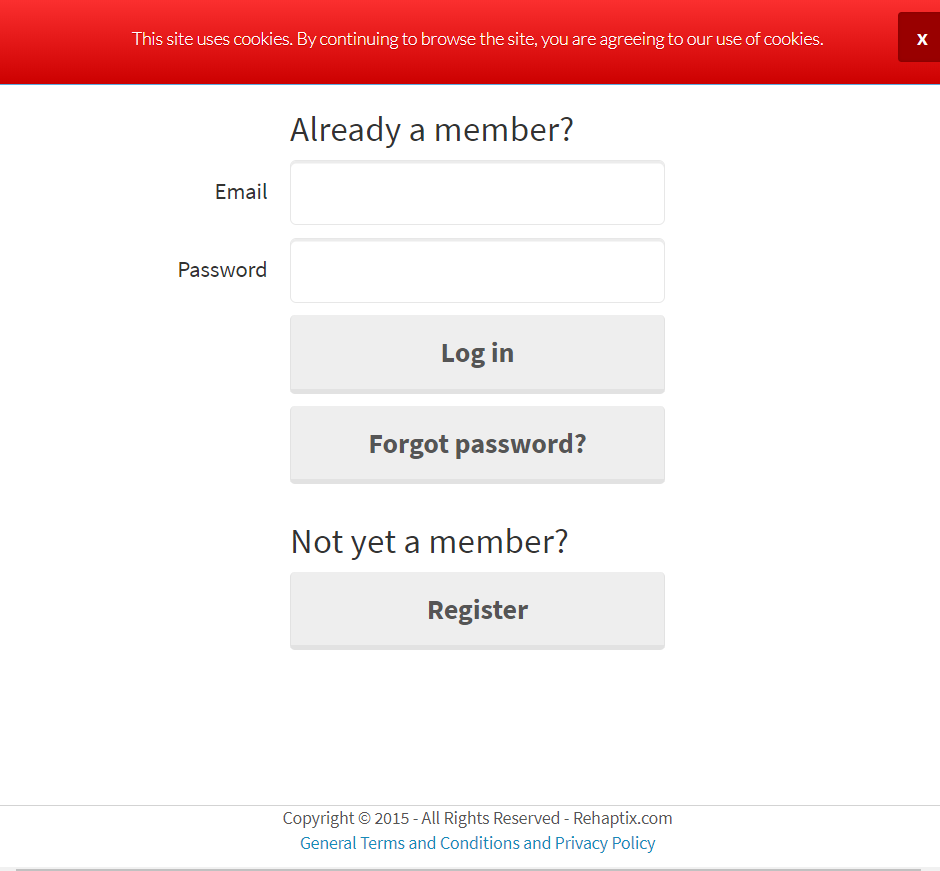
\includegraphics[scale=0.3]{slike/rehaptix2.png}
			\caption{Login}
		\end{figure}


	Kao i naša aplikacija ona omogućava komunikaciju između klijenta i bolnice, prilagođavanje programa rehabilitacije klijentima na temelju njihovog napretka i trenutnog stanja.\\
	Dodatna funckionalnost koju ova aplikacija nudi je testiranje vlastitih sposobnosti.\\
	
	\begin{figure}[h]
	\centering
	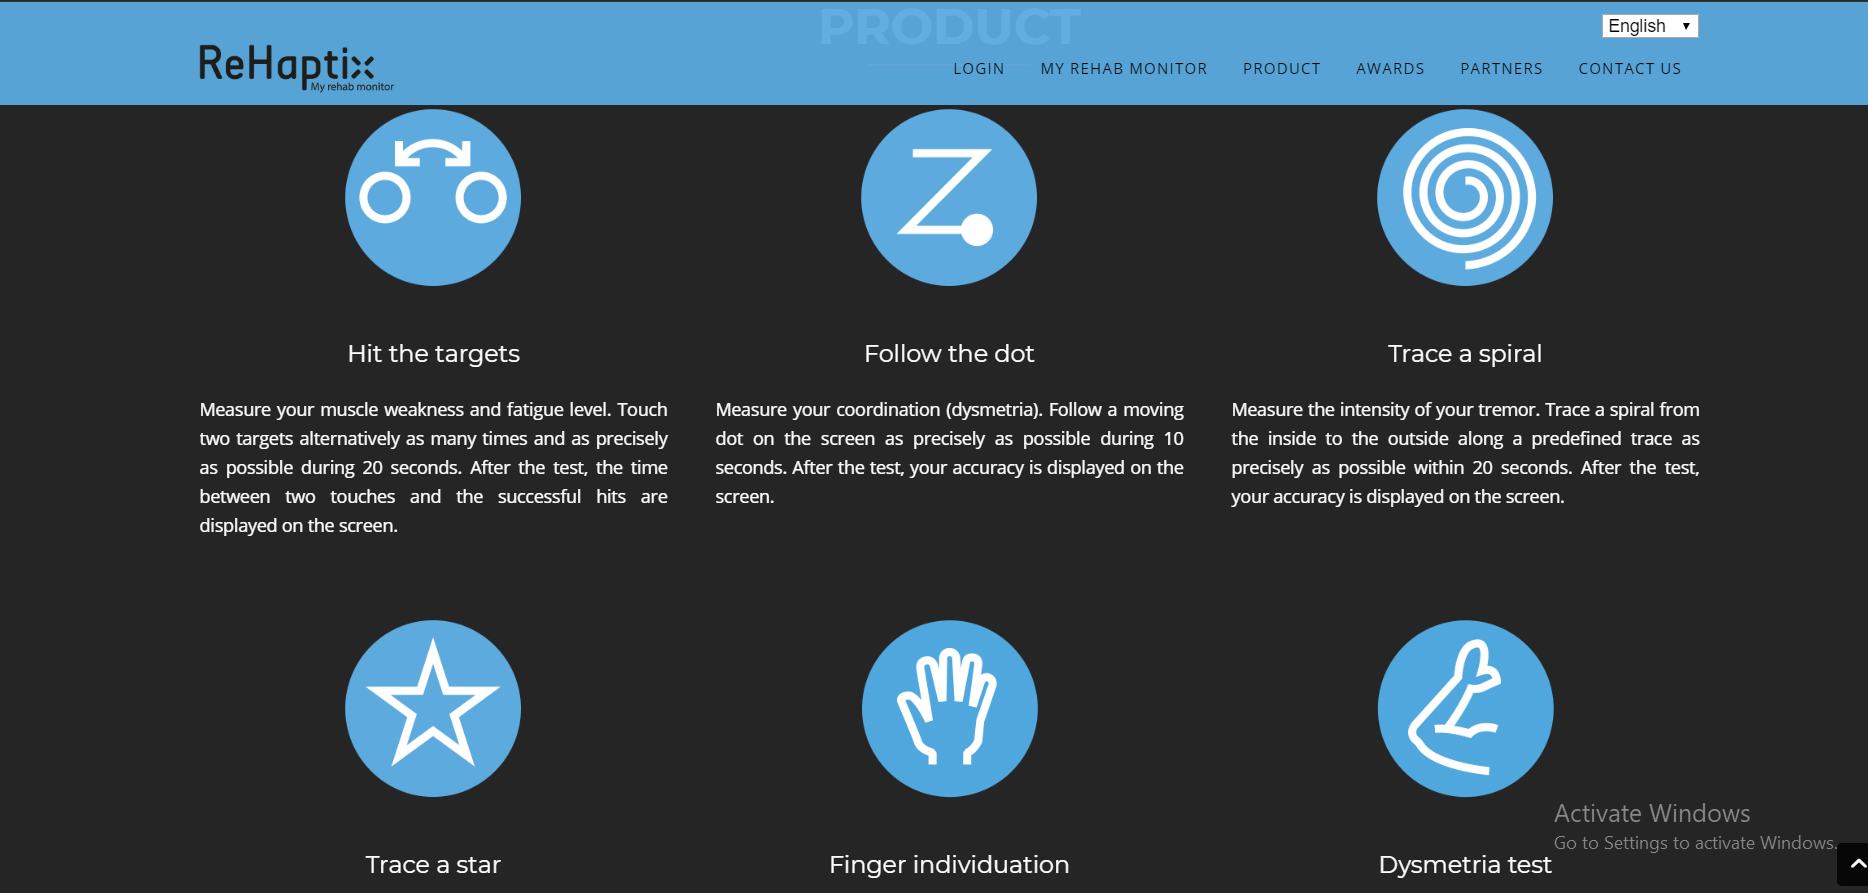
\includegraphics[scale=0.3]{slike/rehaptix3.png}
	\caption{Testiranja}
	\end{figure}

	\begin{figure}[h]
	\centering
	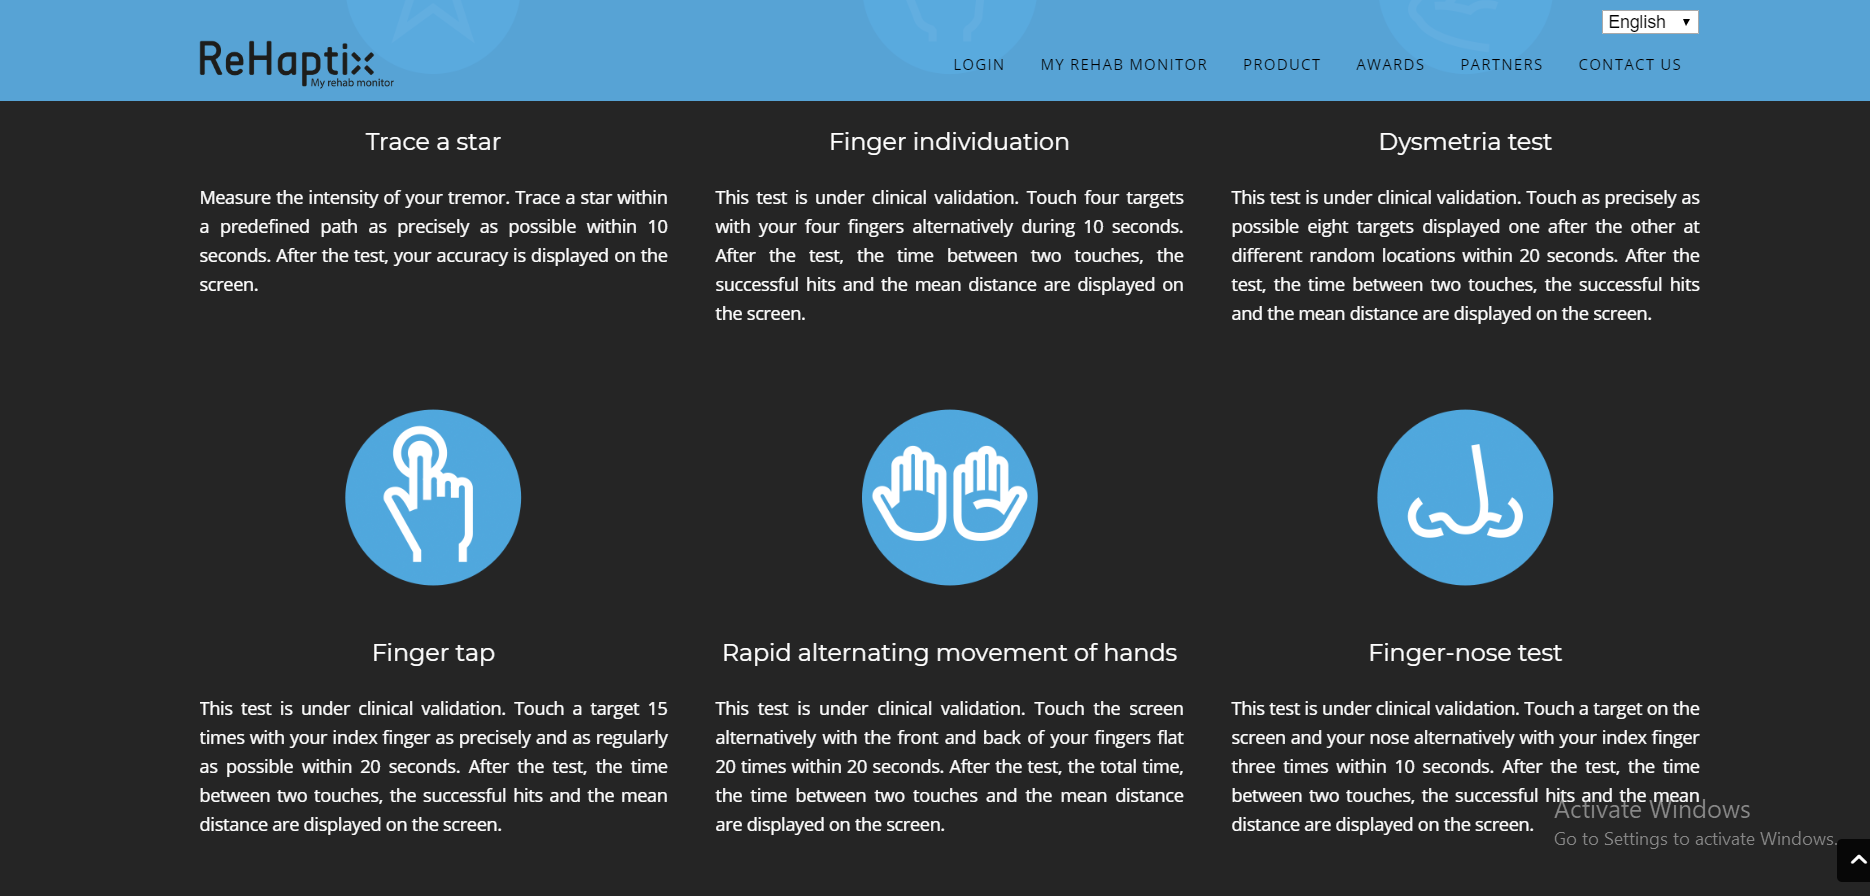
\includegraphics[scale=0.3]{slike/rehaptix4.png}
	\caption{Testiranja}
	\end{figure}

		
		
	\eject
		
	